\usepackage{graphicx,pgf}
\usepackage{tikz}

\mode<article>{\usepackage{fullpage}}

\graphicspath{{images/}}

\beamertemplatetransparentcovered
\usetheme{JuanLesPins}
\useinnertheme{circles}
\useoutertheme[subsection-false]{smoothbars}

\title{Phylogenetics}
\author{Alexei Drummond\only<article>{\footnote{Some content adapted from material provided by Prof Ziheng Yang, UCL}}, alexei@cs.auckland.ac.nz \only<presentation>{\\\quad \\ \tiny{Some slides adapted from material provided by Prof Ziheng Yang, UCL}}}
\date{March 31st, 2009}

\begin{document}


\only<article>{\maketitle}

% TITLE SLIDE
\only<presentation>{

\frame{\titlepage}

%Section1 Outline
\section[Outline]{}}

%Slide1
\frame{\tableofcontents}

%TREE CONCEPTS
\section{Tree Concepts}

%QUIZ
\only<presentation>{\begin{frame}[plain]

\LARGE{

\alert{Quiz}: How many rooted binary trees having 20 labeled terminal nodes are there?  

\medskip{}

(A) 2027025

\medskip{}

(B) 34459425

\medskip{}

(C) $8.20 \times 10^{21}$
 
\medskip{}

(D) $3.21 \times 10^{70}$ 

\bigskip{}

Bonus question: What about unrooted trees?

}

\end{frame}}

%Slide3
%\begin{frame}
%\frametitle{Computational Biology}
%\includegraphics[width=\textwidth]{ComputationalBiology}
%\end{frame}

%MOLECULES AS DOCUMENTS OF HISTORY
\begin{frame}
\frametitle{Molecules as Documents of Evolutionary History}

\begin{itemize}
	\item Macromolecules contain information about the processes and history that formed them
\end{itemize}

\medskip{}

\texttt{HIV-1 (UK.)  ATC\alert{G}GATGCTA\alert{A}AGC\alert{A}TATGA\alert{C}ACAGAGGTACA\alert{TAA}TGTTT}

\texttt{HIV-1 (USA) 	ATC\alert{A}GATGCTA\alert{G}AGC\alert{T}TATGA\alert{T}ACAGAGGTACA\alert{---}TGTTT}

\medskip{}

\begin{itemize}
	\item However, this information is not complete, so the full history must be inferred
	\item One of the aims of computational biology is to decipher the information held in molecular sequences about the process and history of evolution
\end{itemize}

\end{frame}

%PHYLOGENETICS
\begin{frame}
\frametitle{Phylogenetics}

\begin{itemize}
	\item Similarity (homology) is viewed as evidence of common ancestry
	\begin{itemize}
		\item Homology: similarity that is the result of inheritance from a common ancestor
	\end{itemize}
	\item \alert{Phylogenetic trees} are used to portray relationships based upon common ancestry
	\item Monophyletic groups (clades) - contain species which are more closely related to each other than to any outside of the group
	\item Phylogenetics has in recent years become a statistical science based on probabilistic models of evolution (more on this in later lectures).
\end{itemize}
\end{frame}

%A TYPICAL MOLECULAR PHYLOGENETICS ANALYSIS
\begin{frame}
\frametitle{A typical molecular phylogenetics analysis}

\begin{enumerate}
\item Collect homologous sequences
\item Construct a multiple sequence alignment
\item Phylogeny reconstruction
\item Test the reliability of the estimated phylogeny
\item Interpretation and application of phylogenies
\end{enumerate}

\end{frame}

% APPLICATIONS OF PHYLOGENETICS
\begin{frame}
\frametitle{Applications of Phylogenetics}

\begin{itemize}
\item Inferring relationships among species and genes
\item Estimating divergence times
\item Identifying functional elements in comparisons of genomic sequences
\item Detecting molecular adaptation
\item Forensics 
\item Studying the emergence and spread of viral pandemics
\item many more...
\end{itemize}
\end{frame}

% TYPES OF PHYLOGENIES AND REPRESENTATIONS
\begin{frame}
\frametitle{Types of phylogenies and representations}

\begin{columns}

\column{0.66\textwidth}

\begin{centering}

rooted trees

\end{centering}

\column{0.34\textwidth}

\begin{centering}

unrooted tree

\end{centering}

\end{columns}

\begin{columns}[b]

\column{0.33\textwidth}

\begin{centering}

% Auto-generated from TikzTree.java
% xScale=-0.5 yScale=-0.5 offset=0.2
% scalebar=null
% options=[ultra thick]
% newick=((((A: 1, B: 1): 1, C: 2): 1, D: 3): 1, E: 4);
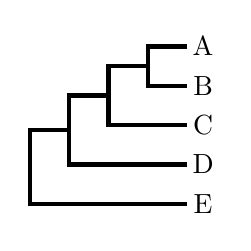
\begin{tikzpicture}[ultra thick]

\node at (0.2, 0.0) {A};
\node at (0.2, -0.5) {B};
\draw (0.0, 0.0) -- (-0.5, 0.0) -- (-0.5, -0.25);
\draw (0.0, -0.5) -- (-0.5, -0.5) -- (-0.5, -0.25);
\node at (0.2, -1.0) {C};
\draw (-0.5, -0.25) -- (-1.0, -0.25) -- (-1.0, -0.625);
\draw (0.0, -1.0) -- (-1.0, -1.0) -- (-1.0, -0.625);
\node at (0.2, -1.5) {D};
\draw (-1.0, -0.625) -- (-1.5, -0.625) -- (-1.5, -1.0625);
\draw (0.0, -1.5) -- (-1.5, -1.5) -- (-1.5, -1.0625);
\node at (0.2, -2.0) {E};
\draw (-1.5, -1.0625) -- (-2.0, -1.0625) -- (-2.0, -1.53125);
\draw (0.0, -2.0) -- (-2.0, -2.0) -- (-2.0, -1.53125);

\end{tikzpicture}

\end{centering}

\bigskip{}

\begin{centering}

(a) cladogram

\end{centering}

\column{0.33\textwidth}

\begin{centering}

% Auto-generated from TikzTree.java
% xScale=-4.0 yScale=-0.5 offset=0.2
% scalebar=scalebar{size= 0.1 visible=true}
% options=[ultra thick]
% newick=((((A: 0.1, B: 0.2): 0.12, C: 0.3): 0.123, D: 0.4): 0.1234, E: 0.5);
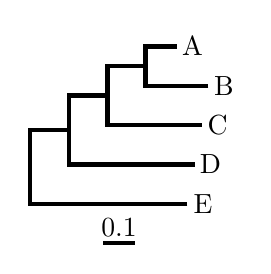
\begin{tikzpicture}[ultra thick]

\node at (-0.2, 0.0) {A};
\node at (0.2, -0.5) {B};
\draw (-0.4, 0.0) -- (-0.8, 0.0) -- (-0.8, -0.25);
\draw (0.0, -0.5) -- (-0.8, -0.5) -- (-0.8, -0.25);
\node at (0.12000000000000001, -1.0) {C};
\draw (-0.8, -0.25) -- (-1.28, -0.25) -- (-1.28, -0.625);
\draw (-0.08, -1.0) -- (-1.28, -1.0) -- (-1.28, -0.625);
\node at (0.028000000000000025, -1.5) {D};
\draw (-1.28, -0.625) -- (-1.772, -0.625) -- (-1.772, -1.0625);
\draw (-0.172, -1.5) -- (-1.772, -1.5) -- (-1.772, -1.0625);
\node at (-0.06559999999999999, -2.0) {E};
\draw (-1.772, -1.0625) -- (-2.2656, -1.0625) -- (-2.2656, -1.53125);
\draw (-0.2656, -2.0) -- (-2.2656, -2.0) -- (-2.2656, -1.53125);

\draw (-0.9328000000000001, -2.5) -- (-1.3328000000000002, -2.5);
\node at (-1.1328, -2.3) {0.1};

\end{tikzpicture}

\end{centering}

\bigskip{}

\begin{centering}

(b) phylogram

\end{centering}

\column{0.33\textwidth}

%\includegraphics[width=\textwidth]{unrootedTree}

\begin{centering}


% Auto-generated from TikzTree.java
% xScale=3.0 yScale=-1.2566370614359172 offset=0.2
% scalebar=scalebar{size= 0.1 visible=true}
% options=[ultra thick]
% newick=((((A: 0.1, B: 0.2): 0.12, C: 0.3): 0.123, D: 0.4): 0.1234, E: 0.5);
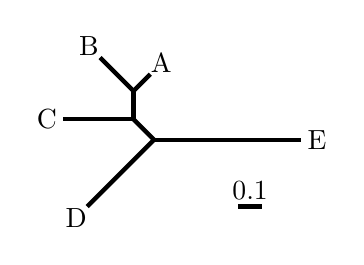
\begin{tikzpicture}[ultra thick]

\node at (-0.27757, 0.97448) {A};
\node at (-1.19681, 1.18661) {B};
\draw (-0.63112, 0.62092) -- (-0.41899, 0.83305);
\draw (-0.63112, 0.62092) -- (-1.05539, 1.04519);
\node at (-1.73112, 0.26092) {C};
\draw (-0.63112, 0.26092) -- (-0.63112, 0.62092);
\draw (-0.63112, 0.26092) -- (-1.53112, 0.26092);
\node at (-1.36015, -0.98995) {D};
\draw (-0.3702, 0) -- (-0.63112, 0.26092);
\draw (-0.3702, 0) -- (-1.21873, -0.84853);
\node at (1.7, -0) {E};
\draw (0, 0) -- (-0.3702, 0);
\draw (0, 0) -- (1.5, -0);

\draw (0.6996, -0.8485281374238571) -- (0.9996, -0.8485281374238571);
\node at (0.8496, -0.6485281374238572) {0.1};

\end{tikzpicture}

(c) unrooted tree

\end{centering}

\end{columns}

\medskip{}

\begin{columns}

\column{0.3\textwidth}

\begin{centering}

\scriptsize{((((A, B), C), D), E);}

\end{centering}

\column{0.7\textwidth}

\begin{centering}

\scriptsize{((((A:0.1, B:0.2):0.12, C:0.3):0.123, D:0.4):0.1234, E:0.5);}

\end{centering}

\end{columns}

\bigskip{}

\begin{centering}

branches (edges) and their lengths, nodes, tips (leaves)

\end{centering}

\end{frame}

%%%%%%%%%%%%%%%%%%%%%%%%%%%%%%%%%%%%%%%%%%
%POLYTOMIES
%%%%%%%%%%%%%%%%%%%%%%%%%%%%%%%%%%%%%%%%%%
\begin{frame}
\frametitle{Bifurcating (binary) and multifurcating trees}

\begin{columns}

\column{0.333\textwidth}

\begin{centering}

% Auto-generated from TikzTree.java
% xScale=2.0 yScale=0.5 offset=-0.2
% scalebar=null
% options=[ultra thick]
% newick=(A:1, B:1, C:1, D:1, E:1);
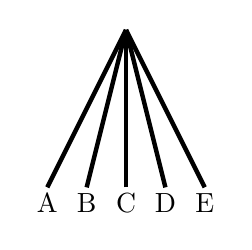
\begin{tikzpicture}[ultra thick]

\node at (0.0, -0.2) {A};
\node at (0.5, -0.2) {B};
\node at (1.0, -0.2) {C};
\node at (1.5, -0.2) {D};
\node at (2.0, -0.2) {E};
\draw (0.0, 0.0) -- (1.0, 2.0);
\draw (0.5, 0.0) -- (1.0, 2.0);
\draw (1.0, 0.0) -- (1.0, 2.0);
\draw (1.5, 0.0) -- (1.0, 2.0);
\draw (2.0, 0.0) -- (1.0, 2.0);

\end{tikzpicture}

star tree

\end{centering}

\column{0.333\textwidth}

\begin{centering}

% Auto-generated from TikzTree.java
% xScale=2.0 yScale=0.5 offset=-0.2
% scalebar=null
% options=[ultra thick]
% newick=((A:0.5, B:0.5):0.5, (C:0.66, D:0.66, E:0.66):0.34);
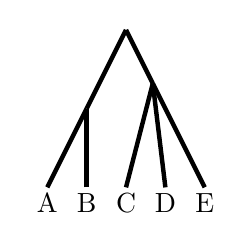
\begin{tikzpicture}[ultra thick]

\node at (0.0, -0.2) {A};
\node at (0.5, -0.2) {B};
\draw (0.0, 0.0) -- (0.5, 1.0);
\draw (0.5, 0.0) -- (0.5, 1.0);
\node at (1.0, -0.2) {C};
\node at (1.5, -0.2) {D};
\node at (2.0, -0.2) {E};
\draw (1.0, 0.0) -- (1.34, 1.32);
\draw (1.5, 0.0) -- (1.34, 1.32);
\draw (2.0, 0.0) -- (1.34, 1.32);
\draw (0.5, 1.0) -- (1.0, 2.0);
\draw (1.34, 1.32) -- (1.0, 2.0);

\end{tikzpicture}

partially-resolved tree

\end{centering}

\column{0.333\textwidth}

\begin{centering}

\input{rootedTree.tex}

fully-resolved tree

\end{centering}

\end{columns}

\medskip{}

\begin{columns}

\column{0.333\textwidth}

\begin{centering}

% Auto-generated from TikzTree.java
% xScale=1.0 yScale=1.2566370614359172 offset=0.2
% scalebar=null
% options=[ultra thick]
% newick=(A:1, B:1, C:1, D:1, E:1);
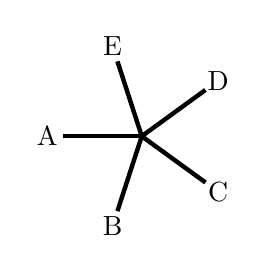
\begin{tikzpicture}[ultra thick]

\node at (-1.2, 0) {A};
\node at (-0.37082, -1.14127) {B};
\node at (0.97082, -0.70534) {C};
\node at (0.97082, 0.70534) {D};
\node at (-0.37082, 1.14127) {E};
\draw (0, 0) -- (-1, 0);
\draw (0, 0) -- (-0.30902, -0.95106);
\draw (0, 0) -- (0.80902, -0.58779);
\draw (0, 0) -- (0.80902, 0.58779);
\draw (0, 0) -- (-0.30902, 0.95106);

\end{tikzpicture}

\end{centering}

\column{0.333\textwidth}

\begin{centering}

% Auto-generated from TikzTree.java
% xScale=1.0 yScale=1.2566370614359172 offset=0.2
% scalebar=null
% options=[ultra thick]
% newick=((A:0.5, B:0.5):0.5, (C:0.66, D:0.66, E:0.66):0.34);
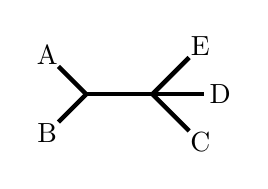
\begin{tikzpicture}[ultra thick]

\node at (-0.99497, 0.49497) {A};
\node at (-0.99497, -0.49497) {B};
\draw (-0.5, 0) -- (-0.85355, 0.35355);
\draw (-0.5, 0) -- (-0.85355, -0.35355);
\node at (0.94811, -0.60811) {C};
\node at (1.2, -0) {D};
\node at (0.94811, 0.60811) {E};
\draw (0.34, -0) -- (0.80669, -0.46669);
\draw (0.34, -0) -- (1, -0);
\draw (0.34, -0) -- (0.80669, 0.46669);
\draw (0, 0) -- (-0.5, 0);
\draw (0, 0) -- (0.34, -0);

\end{tikzpicture}

\end{centering}

\column{0.333\textwidth}

\begin{centering}

\input{unrootedTree.tex}

\end{centering}

\end{columns}

In a rooted tree a \alert{polytomy} is a node with more than 2 children. In an unrooted tree a \alert{polytomy} is a node of degree 4 or greater. 

\end{frame}

%%%%%%%%%%%%%%%%%%%%%%%%%%%%%%%%%%%%%%%%%%
%ROOTED VERSUS UNROOTED TREES
%%%%%%%%%%%%%%%%%%%%%%%%%%%%%%%%%%%%%%%%%%
\begin{frame}
\frametitle{Rooted and unrooted trees}

\begin{columns}[t]

\column{0.333\textwidth}

\begin{centering}

rooted tree

\medskip{}

\input{rootedTree.tex}

\end{centering}

\column{0.667\textwidth}

\begin{centering}

\begin{columns}

\column{0.5\textwidth}

\begin{centering}

\Huge{$\longrightarrow$}

\end{centering}

\column{0.5\textwidth}

\begin{centering}

unrooted tree

\medskip{}

\input{unrootedTree.tex}

\end{centering}

\end{columns}

\end{centering}

\end{columns}

\bigskip{}

Most phylogeny-reconstruction methods are unable to identify the root of the tree, so unrooted trees are inferred.  This includes the maximum parsimony method, as well as distance and likelihood methods that do not assume a molecular clock.

\end{frame}

%Slide7
\begin{frame}
\frametitle{Rooting trees using an outgroup}

\includegraphics[width=\textwidth]{RootingTreesOutgroup}

\end{frame}

% DIFFERENT ROOTINGS OF THE SAME UNROOTED TREE
\begin{frame}
\frametitle{The same unrooted tree}

\includegraphics[width=\textwidth]{unrootedTrees}

These rooted trees all have the same unrooted topology and branch lengths.

\end{frame}


%Slide8
\begin{frame}
\frametitle{Anatomy of a tree}

\includegraphics[width=\textwidth]{AnatomyOfTree}

\end{frame}

%Slide10
\begin{frame}
\frametitle{How many trees are there?}

For $n$ taxa there are

\medskip{}

\begin{centering}

$T^{(R)}_n = (2n - 3)(2n - 5)\dots(3)(1)$ 

\end{centering}

\medskip{}

rooted, binary trees:

\medskip{}

\small{

\begin{tabular}{ccp{0.7\textwidth}} \hline
$n$ & \#trees & \\ \hline
4& 15 &enumerable by hand\\
5& 105 &enumerable by hand on a rainy day\\
6& 945 &enumerable by computer\\
7& 10395 &still searchable very quickly on computer\\
8& 135135 & about the number of hairs on your head\\
9& 2027025 & greater than the population of Auckland\\
10& 34459425 & $\approx$ upper limit for exhaustive search\\
20& $8.20 \times 10^{21}$ & $\approx$ upper limit of branch-and-bound searching\\
48& $3.21 \times 10^{70}$ & $\approx$ the number of particles in the Universe\\
136& $2.11 \times 10^{267}$ & number of trees to choose from in the ``Out of Africa'' data (Vigilante \textit{et al}. 1991)\\
\hline
\end{tabular}

}

%\includegraphics[height=0.5\textheight]{HowManyTrees}

\end{frame}

%COUNTING TREES USING STEPWISE ADDITION ALGORITHM
\begin{frame}
\frametitle{Counting unrooted trees with stepwise addition algorithm}

\includegraphics[width=\textwidth]{stepwiseAddition}

\bigskip{}

%\begin{centering}

$T_3 = 1 \quad \rightarrow \quad T_4 = 1 \times 3 \quad \rightarrow \quad T_5 = 1 \times 3 \times 5$

\medskip{}

$T_n=1\times 3 \times 5 \times \dots \times (2n-5)$ unrooted trees with $n$ leaves

\medskip{}

$T(20)=2.2\times10^{20}, T(53)\approx $ number particles in the universe

%\end{centering}

\end{frame}


%ROBINSON-FOULD DISTANCE SLIDE
\begin{frame}
\frametitle{The topological distance between two trees}

The partition distance (Robinson and Foulds, 1981) is defined as the total number of bipartitions that are in one tree but not in the other.  Each internal branch defines a \alert{bipartition} (\alert{split}) of species.

\medskip{}

\begin{centering}

\includegraphics[width=0.8\textwidth]{robinsonFoulds}

\end{centering}

The distance between those two trees is 2.
The partition distance ranges from 0 to $2(n-3)$ for $n$ species

\end{frame}

%PHYLOGENETIC RECONSTRUCTION SECTION
\section{Phylogenetic reconstruction}

%PHYLOGENETIC RECONSTRUCTIO SLIDE
\begin{frame}
\frametitle{Phylogenetic Reconstruction}

There are essentially two types of data for phylogenetic tree estimation:

\begin{itemize}
	\item \alert{Distance data}, usually stored in a distance matrix, e.g. DNA$\times$DNA hybridisation data, morphometric differences, immunological data, pairwise genetic distances
	\item \alert{Character data}, usually stored in a character array;
	\begin{itemize}
		\item e.g. multiple sequence alignment of DNA sequences, morphological characters.
	\end{itemize}
\end{itemize}

\begin{columns}[t]

\column{.5\textwidth}

\begin{centering}

\scriptsize{

Distances

\medskip{}

\begin{tabular}{c|ccccc}
&A&B&C&D&E \\ \hline
A&0&3&5&6&5\\
B&3&0&4&7&6\\
C&5&4&0&5&4\\
D&6&7&5&0&1\\
E&5&6&4&1&0\\ \hline
\end{tabular}
}

\end{centering}


%\includegraphics[height=0.3\textheight]{Distance}

\column{.5\textwidth}

\begin{centering}

\scriptsize{

Characters

\medskip{}

\begin{tabular}{c|c}
&1 2 3 4 5 6 7 8 9 \\ \hline
A&1 0 0 0 1 1 0 1 1\\
B&0 1 0 0 1 1 1 1 1\\
C&0 0 1 0 0 0 1 1 1\\
D&0 0 0 1 0 0 0 0 0\\
E&0 0 0 0 0 0 0 0 0\\ \hline
\end{tabular}
}

\end{centering}

\end{columns}
\end{frame}

%Slide12
\begin{frame}
\frametitle{Phylogenetic Reconstruction}

 Given the huge number of possible trees even for small data sets, we have two options:
	\begin{itemize}
		\item Build one according to some clustering algorithm
		\item Assign a �goodness of fit� criterion (an objective function) and \alert{find} the tree(s) which optimise(s) this criterion
	\end{itemize}
\end{frame}

%Slide13
\begin{frame}
\frametitle{Phylogenetic Reconstruction}

\includegraphics[width=0.8\textwidth]{PhylogeneticReconstruction}

\end{frame}

\section{Distance-based Algorithms}

%Slide14
\begin{frame}
\frametitle{Clustering Algorithms}

	Common clustering algorithms are \alert{Neighbour-Joining} and \alert{UPGMA} (Unweighted Pair-Group Method using Arithmetic averages).
	
	\bigskip{}
	
	The clustering algorithms are usually very fast, and simple but there is no explicit optimality criterion, so
		\begin{itemize}
			\item we have no measure of how good the tree is!
			\item we do not get any idea about other potential trees - were there any better trees?
		\end{itemize}
		
\end{frame}

%Slide15
\begin{frame}
\frametitle{Clustering Algorithms}

\begin{itemize}
	\item The UPGMA and neighbor-joining (NJ) methods are both greedy heuristics which join, at each step, the two closest* sub-trees that are not already joined.
	\item They are based on the minimum evolution principle.
	\item An important concept in both of these methods is a pair of neighbors, which is defined as two nodes that are connected via a single node:
\end{itemize}

\begin{centering}

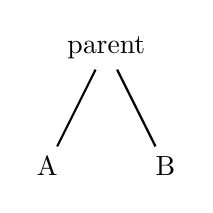
\begin{tikzpicture}[thick] 
\node {parent} 
child { node {A} } 
child {node {B}}; 
\end{tikzpicture} 


%\includegraphics[height=0.2\textheight]{ClusteringAlgorithms}

\end{centering}

\medskip{}

* NJ uses rate-corrected distances

\end{frame}

%Slide16
\begin{frame}
\frametitle{UPGMA Example}

%\includegraphics[height=0.5\textheight]{UPGMAexample1}

\begin{columns}

\column{0.5\textwidth}

\begin{centering}

\begin{tabular}{|c|c|c|c|c|} \hline
&A&B&C&D\\ \hline
A&0&&&\\ \hline
B&8&0&&\\ \hline
C&\textcolor{red}{{\bf 7}}&9&0&\\ \hline
D&12&14&11&0\\ \hline
\end{tabular}

\end{centering}

\column{0.5\textwidth}

\begin{centering}

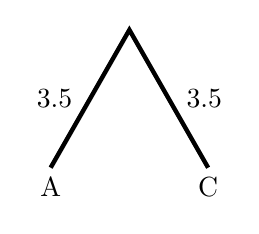
\begin{tikzpicture}[scale=0.5,ultra thick] 

\draw (0,0) -- (2,3.5) -- (4,0);
\node at (0,-0.5) {A}; 
\node at (4,-0.5) {C}; 
\node at (0.1,1.75) {3.5}; 
\node at (3.9,1.75) {3.5}; 
\end{tikzpicture} 

\end{centering}

\end{columns}

\bigskip{}

\begin{centering}

$d_{B(AC)}=(d_{BA}+d_{BC})/2=(8+9)/2=8.5$

\medskip{}

$d_{D(AC)}=(d_{DA}+d_{DC})/2=(12+11)/2=11.5$

\end{centering}
\end{frame}

%Slide17
\begin{frame}
\frametitle{UPGMA Example}

%\includegraphics[height=0.5\textheight]{UPGMAexample2}

\begin{columns}

\column{0.5\textwidth}

\begin{centering}

\begin{tabular}{|c|c|c|c|} \hline
&AC&B&D\\ \hline
AC&0&&\\ \hline
B&\textcolor{red}{{\bf 8.5}}&0&\\ \hline
D&11.5&14&0\\ \hline
\end{tabular}

\end{centering}

\column{0.5\textwidth}

\begin{centering}

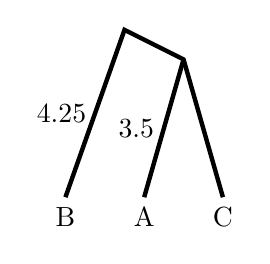
\begin{tikzpicture}[scale=0.5,ultra thick] 

\draw (0,0) -- (1.5,4.25) -- (3,3.5) -- (4,0);
\draw (2,0) -- (3,3.5);
\node at (0,-0.5) {B}; 
\node at (2,-0.5) {A}; 
\node at (4,-0.5) {C}; 
\node at (-0.1,2.125) {4.25}; 
\node at (1.8,1.75) {3.5}; 
\end{tikzpicture} 

\end{centering}

\end{columns}

\bigskip{}

\begin{centering}
$d_{(ABC)D}=(d_{AD}+d_{BD}+d_{CD})/3=(12+14+11)/3\approx12.33$
\end{centering}

\end{frame}

%Slide18
\begin{frame}
\frametitle{UPGMA Example}

%\includegraphics[height=0.5\textheight]{UPGMAexample3}

\begin{columns}

\column{0.5\textwidth}

\begin{centering}

\begin{tabular}{|c|c|c|c|} \hline
&ABC&D\\ \hline
ABC&0&\\ \hline
D&\textcolor{red}{{\bf 12.33}}&0\\ \hline
\end{tabular}

\end{centering}

\column{0.5\textwidth}

\begin{centering}

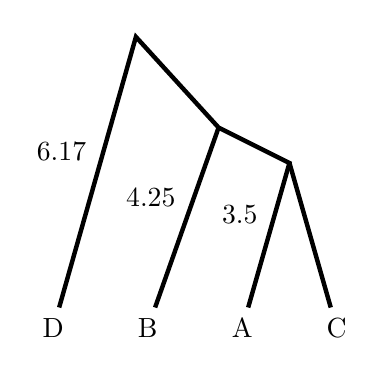
\begin{tikzpicture}[scale=0.6,ultra thick] 

\node (D) at (0,0) {D}; 
\node (B) at (2,0) {B}; 
\node (A) at (4,0) {A}; 
\node (C) at (6,0) {C}; 
\node (AC) at (5,3.5) {};
\node (ABC) at (3.5,4.25) {};
\node (ABCD) at (1.75,6.17) {};

\draw (C) to (AC.center);
\draw (B) to node[auto] {4.25} (ABC.center);
\draw (D) to node[auto] {6.17} (ABCD.center)  to
 (ABC.center) to (AC.center) to node[auto, swap] {3.5} (A);

\end{tikzpicture} 

\end{centering}

\end{columns}

\bigskip{}

UPGMA produces a \alert{rooted tree} and assumes that evolution is \alert{clock-like}, i.e. it assumes that the rate of substitution is the same on all branches of the tree

\end{frame}

%%%%%%%%%%%%%%%%%%%%%%%%%%%%%%%%
% UPGMA WEAKNESSES
%%%%%%%%%%%%%%%%%%%%%%%%%%%%%%%%
\begin{frame}
\frametitle{UPGMA weaknesses}

%\includegraphics[height=0.5\textheight]{UPGMAexample4}

\begin{columns}

\column{0.5\textwidth}

\begin{centering}

\begin{tabular}{|c|c|c|c|c|} \hline
&A&B&C&D\\ \hline
A&0&&&\\ \hline
B&8&0&&\\ \hline
C&7&9&0&\\ \hline
D&12&14&11&0\\ \hline
\end{tabular}

\end{centering}

\column{0.5\textwidth}

\begin{centering}

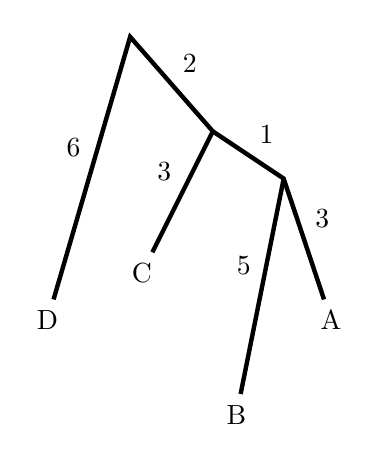
\begin{tikzpicture}[scale=0.6,ultra thick] 

\node (D) at (0,0) {D}; 
\node (C) at (2,1) {C}; 
\node (B) at (4,-2) {B}; 
\node (A) at (6,0) {A}; 
\node (AB) at (5,3) {};
\node (ABC) at (3.5,4) {};
\node (ABCD) at (1.75,6) {};

\draw (B) to node[auto] {5} (AB.center);
\draw (C) to node[auto] {3} (ABC.center);
\draw (D) to node[auto] {6} (ABCD.center)  to node[auto] {2}
 (ABC.center) to node[auto] {1} (AB.center) to node[auto] {3} (A);
%\draw (2,-3) -- (3,2);
%\draw (-2,-1) -- (-0.25,5) -- (1.5,3);

\end{tikzpicture} 

\end{centering}

\end{columns}

\medskip{}

There is a (non clock-like) tree that fits the distance matrix exactly!

\end{frame}

%Slide21
\begin{frame}
\frametitle{Neighbor-joining algorithm (Saitou and Nei, 1987)}

\begin{itemize}
	\item Most widely-used distance-based method for phylogenetic reconstruction
	\item UPGMA illustrated that it is not enough to pick the closest neighbors (at least when there is rate heterogeneity across branches)
	\item Idea: take into account averaged distances to other leaves as well
	\item Produces an unrooted tree
\end{itemize}

\end{frame}

%Slide22
\begin{frame}
\frametitle{The basic idea}

\begin{itemize}
	\item We start by computing the ``average distance'' from $i$ to every other taxon

\begin{centering}

$r_i=\frac{1}{n-2} \sum_j d_{ij}$

\end{centering}

\medskip{}

	\item We then compute new corrected distances for all pairs of $(i,j)$:

\medskip{}

\begin{centering}

$d^{*}_{ij}=d_{ij}-r_i-r_j$

\end{centering}

\medskip{}

	\item We are effectively pushing each node $i$ closer to all other nodes by $r_i$.
\end{itemize}

\end{frame}

%Slide23
\begin{frame}
\frametitle{The basic idea}

\begin{centering}

$d^{*}_{ij}=d_{ij}-r_i-r_j$

\end{centering}

\bigskip{}

The effect is to correct for long branches.

\bigskip{}


\begin{columns}

\column{0.5\textwidth}

\begin{centering}

% Auto-generated from TikzTree.java
% xScale=0.3 yScale=-1.5707963267948966 offset=0.2
% scalebar=null
% options=[ultra thick]
% newick=((A:3.0,B:5.0):1.0,C:3.0,D:8.0);
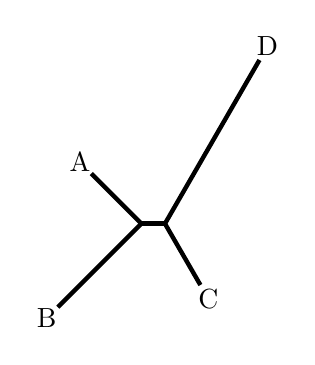
\begin{tikzpicture}[ultra thick]

\node at (-1.07782, 0.77782) {A};
\node at (-1.50208, -1.20208) {B};
\draw (-0.3, 0) -- (-0.9364, 0.6364);
\draw (-0.3, 0) -- (-1.36066, -1.06066);
\node at (0.55, -0.95263) {C};
\node at (1.3, 2.25167) {D};
\draw (0, 0) -- (-0.3, 0);
\draw (0, 0) -- (0.45, -0.77942);
\draw (0, 0) -- (1.2, 2.07846);

\end{tikzpicture}

\end{centering}

\column{0.5\textwidth}

\scriptsize{
$d= 
 \begin{bmatrix}
  0 & 8 &7 & 12 \\
  8 & 0 & 9 & 14 \\
  7  & 9  & 0 & 11  \\
  12 & 14 & 11 & 0
 \end{bmatrix}$
}
\medskip{}

\scriptsize{
$r = [13.5, 15.5, 13.5, 18.5]$
}
\medskip{}

\scriptsize{
$d^{*}= 
 \begin{bmatrix}
  0 & -21 & -20 & -20 \\
  -21 & 0 & -20 & -20 \\
  -20  & -20  & 0 & -21  \\
  -20 & -20 & -21 & 0
 \end{bmatrix}$
}

\end{columns}

\medskip{}

\normalsize{
This is the result of the Neighbor-joining algorithm on same distance matrix as used in the UPGMA example. $AB$ and $CD$ are grouped instead of $AC$.
}

\end{frame}

%Slide24
\begin{frame}
\frametitle{Neighbor-joining}

\begin{itemize}
	\item We use an algorithm very similar to UPGMA to select the two closest nodes, $i$ and $j$, based on the corrected distances ($d^{*}$).
	\item We join these into a cluster and make a new node $k$ to correspond to their ancestor
	\item the distance to the new node $k$ is computed by $d_{ik} = \frac{1}{2}(d_{ij} + r_i - r_j)$
	
	\item Nodes $i$ and $j$ are removed from the pool and replaced by $k$. The uncorrected distances are updated based on the $d_{ik}$ calculation and $d^{*}$ is then recalculated.
	\item See Higgs and Attwood (2005; pp166-169) for details. 
\end{itemize}

\end{frame}

% TIME COMPLEXITY OF CLUSTERING ALGORITHMS
\begin{frame}
\frametitle{Time complexity of the clustering algorithms}

\begin{itemize}
	\item Both of these clustering-based algorithms take $O(n^{3})$ time once we have the distance matrix.
	\item There are $n$ steps and in each step we do:

(1) find the smallest distance

(2) join these two taxa

(3) compute the distance from the new ancestor to all others

	\item Step (1) takes $O(n^{2})$ and the other two steps take $O(n)$
\end{itemize}

\bigskip{}

Note: There is an alternative (and much harder to follow) formulation of the UPGMA algorithm that takes $O(n^2)$

\end{frame}

% LEAST SQUARES 1
\begin{frame}
\frametitle{Least squares distance-based phylogenetics}

\begin{tabular}{|c|c|c|c|c|} \hline
$d_{ij}$&Human&Chimp&Gorilla&Orangutan\\ \hline
Human&0&&&\\ \hline
Chimp&0.0965&0&&\\ \hline
Gorilla&0.1140&0.1180&0&\\ \hline
Orangutan&0.1849&0.2009&0.1947&0\\ \hline
\end{tabular}

\begin{columns}

\column{0.3\textwidth}

\begin{centering}

\includegraphics[width=\textwidth]{hcgoTree}

\end{centering}

\column{0.7\textwidth}

\begin{align*}
S = &(d_{12} - \hat{d}_{12})^2 + (d_{13} - \hat{d}_{13})^2 + \\ 
&(d_{14} - \hat{d}_{14})^2 + (d_{23} - \hat{d}_{23})^2 + \\
&(d_{24} - \hat{d}_{24})^2 + (d_{34} - \hat{d}_{34})^2 \end{align*}

\medskip{}

$\hat{d}_{12} = t_1 + t_2, \quad \hat{d}_{13} = t_1 + t_0 + t_3, \dots$

\end{columns}

\bigskip{}

There are six data points (distances) and five free parameters (branch lengths).

\end{frame}

% LEAST SQUARES 2
\begin{frame}
\frametitle{Least squares distance-based phylogenetics}

\scriptsize{
\begin{tabular}{|c|c|c|c|c|c|c|} \hline
Tree&$t_0\footnote{internal branch}$&$t_1$ (H)&$t_2$ (C)&$t_3$ (G)&$t_4$ (O)&S\\ \hline
((H,C),G,O)&0.008840&0.043266&0.053280&0.058908&0.135795&0.000035\\ \hline
((H,G),C,O)&0.0&0.46212&0.056227&0.061854&0.138742&0.000140\\ \hline
((H,O),C,G)&0.0&0.46212&0.056227&0.061854&0.138742&0.000140\\ \hline
(H,G,C,O)&0.0&0.46212&0.056227&0.061854&0.138742&0.000140\\ \hline
\end{tabular}
}

\bigskip{}

\begin{centering}

\includegraphics[width=0.8\textwidth]{leastSquares}

\end{centering}


\end{frame}

%READING FOR TREE CONCEPTS AND DISTANCE METHODS
\begin{frame}
\frametitle{Reading: Trees and Distance Methods}

\begin{itemize}
\item Bioinformatics and Molecular Evolution, Higgs and Attwood (2005), sections 8.1 and 8.3
\item Computational Molecular Evolution, Ziheng Yang (2006), sections 3.1-3.3
\item Biological Sequence Analysis, Durbin \textit{et al} (1998), sections 7.1-7.3
\item An Introduction to Bioinformatics Algorithms, Jones and Pevzner (2004), Chapter 10
\end{itemize}

\end{frame}

\end{document}
